\documentclass[11pt]{article}
\usepackage[margin=1in]{geometry}
\usepackage{amsmath,amssymb}
\usepackage{booktabs}
\usepackage{graphicx}
\usepackage[numbers,sort&compress]{natbib}
\usepackage{xcolor}
\usepackage[colorlinks=true,linkcolor=blue!50!black,citecolor=blue!50!black,urlcolor=blue!50!black]{hyperref}
\usepackage{microtype}

\newcommand{\kappaworst}{2,356}
\newcommand{\kappadata}{202}


\title{When the Safeguard Is the Failure:\\Uncertainty-Based Termination in Model-Based Offline RL\\on a Simulated Process-Control Task}
\author{Artem Zvyagintsev\\[2pt]\small Independent researcher\\\small\texttt{artem.zvyagintsev@gmail.com}}
\date{}

\begin{document}
\maketitle

\begin{abstract}
Model-based offline reinforcement learning methods such as MOReL guard against model exploitation by terminating synthetic rollouts, with a large penalty, wherever an ensemble's disagreement exceeds a threshold. We study this mechanism on a simulated industrial coating process with an integrating tank level and a transport delay, using ten seeds, paired comparisons and a confirmation run on ten fresh seeds. MOReL with a hybrid physics-plus-residual dynamics model is unstable, and a $2\times2$ factorial ablation locates the cause: with termination switched off, the learned model is as good as the true dynamics for policy learning (paired difference $+0.001$ [$-0.002$, $+0.004$]) and the agent, then plain model-based SAC, beats CQL by $+0.19$ [$+0.15$, $+0.23$]; with termination on, even the true dynamics produce failing seeds. Two design choices explain the damage. A threshold set at a percentile of the uncertainty on the data halts that share of in-distribution transitions by construction, and a penalty sized to deter halting in the worst case is three orders of magnitude larger than ordinary rewards, so that a few percent of halted rollouts dominate the critic. Raising the threshold to the 99th percentile removes the failing seeds but leaves the agent worse than behavioral cloning; taking the penalty from the data instead recovers most of the loss, but no termination setting we tried beats none. Multi-step diagnostics show why the uncertainty is a poor trigger: over a 20-step rollout the model's error grows five- to sixfold while the ensemble's disagreement stays flat, and its rank correlation with the error falls from 0.4 to near zero. The results concern one simulated process and one rollout horizon; they argue for measuring a pessimism mechanism like any other component rather than for dropping pessimism in general. Code, results and a companion book are public.
\end{abstract}

\section{Introduction}

Offline reinforcement learning learns a policy from logged data without trial actions on the system~\citep{levine2020offline}. Its central risk is extrapolation: a learned value function or dynamics model can be wrong where the data are thin, and an optimizer will find those errors. Model-based offline methods answer with pessimism built on an uncertainty estimate. MOPO subtracts a penalty proportional to the uncertainty from the reward~\citep{yu2020mopo}; MOReL builds a pessimistic MDP in which any state-action pair whose uncertainty exceeds a threshold $\epsilon$ leads to an absorbing HALT state with a large penalty $\kappa$~\citep{kidambi2020morel}. The uncertainty is usually the disagreement of an ensemble of learned models~\citep{lakshminarayanan2017ensembles,chua2018pets}.

These safeguards are rarely tested on their own. Benchmarks report the full algorithm, and when a model-based method underperforms, the usual suspect is the model. We report a case where that diagnosis was wrong. On a simulated coating process with an integrating level and a transport delay, MOReL with a hybrid physics-plus-residual model failed on some seeds, and the physics prior was demonstrably wrong on one control loop, which made the model the natural culprit. A factorial ablation showed instead that the model was adequate and the termination rule caused the failures.

Our contributions are empirical and methodological:
\begin{itemize}
  \item A $2\times2$ ablation crossing learned versus true dynamics with HALT on versus off, which separates model error from the pessimism mechanism (Section~\ref{sec:factorial}).
  \item A study of the termination rule: threshold percentile and the size of $\kappa$, on two versions of the state, one of them non-Markov with a wrong physics prior (Section~\ref{sec:halt}).
  \item One-step and multi-step diagnostics of whether ensemble disagreement tracks the model's actual error, using the true dynamics as an oracle (Section~\ref{sec:uncertainty}).
  \item A confirmation of the main conclusions on ten seeds that played no part in choosing the configurations (Section~\ref{sec:fresh}).
\end{itemize}
All experiments use ten seeds, Student-$t$ intervals over per-seed means and paired per-seed differences, following the advice of~\citet{henderson2018matters} and \citet{agarwal2021precipice} on reporting uncertainty in RL results.

\section{Related work}

MOReL~\citep{kidambi2020morel} and MOPO~\citep{yu2020mopo} introduced the two standard forms of uncertainty-based pessimism in model-based offline RL. Both rely on an uncertainty estimate whose admissibility --- that it bounds the model's error --- is assumed rather than guaranteed. COMBO~\citep{yu2021combo} removes the explicit uncertainty estimate and applies CQL-style value regularization~\citep{kumar2020cql} to model-generated transitions instead. MBPO~\citep{janner2019mbpo} uses short model rollouts branched from real states, without pessimism, in the online setting; the agent we obtain by switching HALT off is essentially MBPO trained on a fixed dataset. Closest to our study, \citet{lu2022revisiting} revisit design choices in offline model-based RL, including the choice of uncertainty heuristic, the penalty weight and the rollout length, and show that they interact strongly with performance; our factorial design isolates one such choice, termination, on a process-control task. Industrial and near-real-world offline benchmarks such as the Industrial Benchmark~\citep{hein2017industrial} and NeoRL~\citep{qin2022neorl} share features of our task --- narrow logs from conservative controllers, delays, partial observability --- that standard locomotion suites~\citep{fu2020d4rl} lack.

\section{Setup}

\paragraph{Process.} A simulated coating line has five measured variables: temperature $T$, filler fraction $f$, viscosity $v$, density $d$ and surge-tank level $L$, all in $[0,1]$, and two actuator commands in $[-1,1]$, heater and feed. Temperature and filler follow first-order dynamics, $T$ with a cross-coupling to the filler and $f$ with a two-step transport delay, $f_{t+1}$ depending on the feed command $u_{f,t-2}$; viscosity and density are algebraic (viscosity nonlinear) functions of $T$ and $f$; the level integrates the difference between the feed and a fixed downstream demand, so it has no equilibrium of its own and shares its only actuator with the filler loop. Measurements carry Gaussian noise. The reward penalizes squared deviations of $T$, $f$ and $L$ from their setpoints and the squared actions. Hard bounds on all five variables define constraint violations.

\paragraph{State.} Because of the delay, the five measured variables are not a Markov state. We run every experiment on two versions: the five variables as an operator's historian would log them, and an augmented state with the two feed commands in transit, $(s_t, u_{f,t-2}, u_{f,t-1})$, which is Markov.

\paragraph{Data.} Each seed generates 400 episodes of 100 steps (40{,}000 transitions) from noisy proportional operators that leave steady-state offsets: 60\% normal operation, 25\% setpoint transitions, 15\% disturbances with a low tank level. Episodes end on a time limit, which is not treated as termination in the TD targets.

\paragraph{Methods.} Behavioral cloning (BC); CQL~\citep{kumar2020cql} with $\alpha=1$; CQL with a reward penalty for leaving the bounds; and MOReL~\citep{kidambi2020morel} with a hybrid dynamics ensemble. The hybrid ensemble has four members, each predicting a known first-order physics model plus a learned Gaussian residual; on the Markov state the physics applies the delay exactly, on the logged state it cannot, and it then predicts the filler increments worse than predicting no change (explained variance $-50\%$). The policy is optimized with SAC~\citep{haarnoja2018sac} on batches that are half real transitions and half transitions from five-step model rollouts branched from dataset states, 15 outer iterations of 300 gradient steps. The HALT threshold $\epsilon$ is a percentile of the ensemble's disagreement on dataset transitions; the default is the 80th percentile, and the default penalty is $\kappa = \max(100,\ 2\max|r|/(1-\gamma))$ with $\gamma=0.99$, the value of staying forever in the worst-rewarded state, doubled ($\approx\kappaworst$ in normalized reward units). The same agent with the true noise-free dynamics in place of the ensemble serves as an oracle.

\paragraph{Evaluation.} Each policy runs 20 episodes of 200 steps on the real (simulated) process, half from nominal and half from disturbed starts. We report the mean return, the integrated absolute error (IAE) of the level and the number of failing seeds, defined as a mean return below $-10$ (an order of magnitude below every stable configuration). Intervals are 95\% Student-$t$ intervals over the ten per-seed means; comparisons between methods are paired by seed, since within a seed all methods see the same dataset.

\section{Results}

\subsection{Baseline comparison}

Table~\ref{tab:benchmark} reports the four methods on both versions of the state. CQL clearly improves on BC, mostly by removing the operators' steady-state offsets, and the bounds penalty adds a small gain detectable only in a paired comparison ($+0.07$ [$+0.03$, $+0.10$] on the Markov state). MOReL is the worst method on average and has a failing seed on the logged state, where its physics prior is wrong.

\begin{table}[h]
\centering\small
\resizebox{\linewidth}{!}{%
\begin{tabular}{lcccccc}
\toprule
& \multicolumn{3}{c}{Five logged variables} & \multicolumn{3}{c}{Markov state} \\
\cmidrule(lr){2-4}\cmidrule(lr){5-7}
Method & Return & Level IAE & Fails & Return & Level IAE & Fails \\
\midrule
\csname @@input\endcsname tables/benchmark.tex \bottomrule
\end{tabular}}
\caption{Benchmark, ten seeds (0--9). Return over 200 steps, mean [95\% $t$-interval]; a seed fails when its mean return is below $-10$.}
\label{tab:benchmark}
\end{table}

\subsection{Model or termination rule?}\label{sec:factorial}

Table~\ref{tab:factorial} crosses the dynamics (learned hybrid or true) with the termination rule (HALT at the 80th percentile or none), on the Markov state, with the same SAC budget, rollout horizon, reward and policy initialization in every cell. Without HALT the learned model is as good as the truth for policy learning: the paired difference between the two right-hand cells is $+0.001$ \,[$-0.002$, $+0.004$]%
, and both beat CQL on the same datasets. With HALT, the learned model has two failing seeds and the true dynamics one, with a return of $-224$. The termination rule, not the model, is the bottleneck, and the policy-optimization budget is not the problem either, since the same 4{,}500 SAC steps suffice once HALT is off. Note that the agent without HALT and without any uncertainty penalty is no longer MOReL: it is model-based SAC with no pessimism, close to MBPO~\citep{janner2019mbpo} on a fixed dataset.

\begin{table}[h]
\centering\small
\resizebox{\linewidth}{!}{%
\begin{tabular}{llcccc}
\toprule
Dynamics & HALT & Return & Level IAE & Fails & Paired vs CQL \\
\midrule
\csname @@input\endcsname tables/factorial.tex \bottomrule
\end{tabular}}
\caption{Factorial ablation on the Markov state, seeds 0--9. ``Paired vs CQL'' is the per-seed return difference against CQL trained on the same dataset.}
\label{tab:factorial}
\end{table}

\subsection{Threshold and penalty}\label{sec:halt}

A percentile threshold labels a fixed share of in-distribution transitions UNKNOWN: at the 80th percentile, about 22\% of rollout steps halt. Each halt costs $\kappa\approx\kappaworst$ against ordinary rewards near $-1$, so a fifth of the synthetic data carries a penalty three orders of magnitude larger than anything else, and the critic's targets are set by where the threshold happens to fall. Table~\ref{tab:halt} varies the rule with the learned model held fixed. Raising the threshold to the 99th percentile cuts the halt rate to about 5\% and removes the failing seeds, but the agent remains worse than BC. Keeping the 99th percentile and taking $\kappa$ from the data instead --- the magnitude of the most negative discounted return-to-go in the logs, about \kappadata --- improves the return by $+2.66$ \,[$+1.82$, $+3.50$]
, to between BC and CQL. No termination setting beats none. On the logged state, where the physics prior is wrong on the filler loop, the picture is the same: the failures come from HALT, and without it the agent still beats CQL. The physics error mattered much less to the final policy than to the one-step predictions.

\begin{table}[h]
\centering\scriptsize
\setlength{\tabcolsep}{3pt}
\resizebox{\linewidth}{!}{%
\begin{tabular}{lcccccccc}
\toprule
& \multicolumn{4}{c}{Markov state} & \multicolumn{4}{c}{Five logged variables} \\
\cmidrule(lr){2-5}\cmidrule(lr){6-9}
Termination & Return & Halted & Fails & vs CQL & Return & Halted & Fails & vs CQL \\
\midrule
\csname @@input\endcsname tables/halt.tex \bottomrule
\end{tabular}}
\caption{Termination rule with the learned hybrid model fixed, seeds 0--9. ``Halted'' is the mean share of rollout steps that reach HALT. The data-derived $\kappa$ was run on the Markov state only.}
\label{tab:halt}
\end{table}

\subsection{Does the uncertainty track the error?}\label{sec:uncertainty}

The oracle gives the model's actual error anywhere. One step ahead, on 4{,}000 dataset states per seed, the ensemble's disagreement is informative but weakly (Table~\ref{tab:calibration}): its rank correlation with the error is about 0.4, the quintile with the highest disagreement has about twice the error of the lowest, and pairs labelled KNOWN at the 80th-percentile threshold keep more than half the error of pairs labelled UNKNOWN.

\begin{table}[h]
\centering\small
\resizebox{\linewidth}{!}{%
\begin{tabular}{lcccc}
\toprule
Actions & Spearman($u$, error) & Error, lowest / highest $u$ quintile & Error, KNOWN / UNKNOWN & Share KNOWN \\
\midrule
\csname @@input\endcsname tables/calibration.tex \bottomrule
\end{tabular}}
\caption{One-step error of the hybrid ensemble against the true dynamics (Euclidean norm over the five process variables, normalized units), mean over seeds.}
\label{tab:calibration}
\end{table}

Over several steps it says almost nothing (Table~\ref{tab:rollout}, Figure~\ref{fig:rollout}). From 400 random dataset states per seed, the model and the true dynamics follow either the same logged action sequence (open loop) or the trained policy acting on each trajectory's own states (closed loop). The model's error grows five- to sixfold over 20 open-loop steps and about threefold in closed loop, while the disagreement $u$ --- the ensemble's one-step disagreement at the current predicted state --- stays flat, and its rank correlation with the error falls to near zero by step 10. The members drift together, so their disagreement does not grow with the accumulated error. HALT therefore fires mostly at the first step, on transitions that are in the data, and rarely where the model has actually drifted. No rollout is stopped in this diagnostic; ``halted by step $k$'' counts rollouts whose disagreement has exceeded $\epsilon$ at least once by step $k$.

\begin{table}[h]
\centering\small
\resizebox{\linewidth}{!}{%
\begin{tabular}{cccccc}
\toprule
Step $k$ & Error, open loop & Error, closed loop & Mean $u$ & Halted by $k$ (open / closed) & Spearman($u$, error) (open / closed) \\
\midrule
\csname @@input\endcsname tables/rollout.tex \bottomrule
\end{tabular}}
\caption{Multi-step error of the hybrid model against the true dynamics (root-mean-square over start states of the Euclidean error, normalized units), mean over seeds. MOReL's rollouts use $k\le5$.}
\label{tab:rollout}
\end{table}

\begin{figure}[h]
\centering
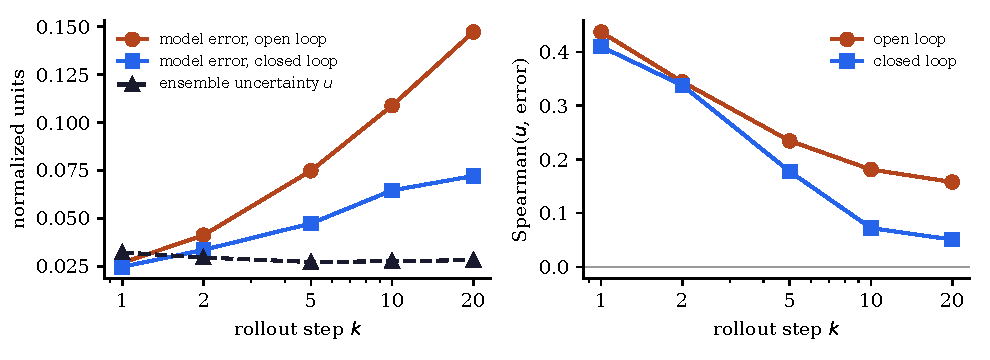
\includegraphics[width=\linewidth]{figures/rollout_error.pdf}
\caption{Left: the model's multi-step error grows while the ensemble's disagreement does not. Right: the rank correlation between disagreement and error decays with the rollout step.}
\label{fig:rollout}
\end{figure}

The policy did not exploit these multi-step errors: without HALT it did as well on the learned model as on the truth. With five-step rollouts and half of every batch real data, the errors stayed small enough not to matter.

\subsection{Confirmation on fresh seeds}\label{sec:fresh}

The configurations above were compared, and the conclusions drawn, on seeds 0--9, which makes the comparison exploratory. We therefore reran the benchmark and the termination study on the Markov state for ten new seeds, 10--19 (Table~\ref{tab:fresh}). Every conclusion held: the agent without HALT beat CQL by $+0.21$ [$+0.18$, $+0.24$]; the 80th-percentile threshold again produced two failing seeds; the data-derived $\kappa$ again landed between BC and CQL; and the bounds penalty again improved on CQL.

\begin{table}[h]
\centering\small
\resizebox{\linewidth}{!}{%
\begin{tabular}{lccc}
\toprule
Method & Return & Fails & Paired vs CQL \\
\midrule
\csname @@input\endcsname tables/fresh.tex \bottomrule
\end{tabular}}
\caption{Confirmation on fresh seeds 10--19, Markov state.}
\label{tab:fresh}
\end{table}

\section{Discussion}

\paragraph{Why the safeguard failed.} Two choices that look conservative combined into the dominant training signal. A percentile threshold guarantees that a fixed share of in-distribution transitions halts, whatever the model's actual error; a penalty sized for the worst case guarantees that each halt outweighs everything else the critic sees. Neither is specific to our task, and both are common defaults. The data-derived penalty shows that the size of $\kappa$ matters as much as the threshold. Its residual cost --- the agent still trails the version without termination --- is consistent with the diagnostics: an uncertainty that barely tracks the model's error cannot direct the halts to where they would help.

\paragraph{What this does not show.} Pessimism was unnecessary here because the model was accurate enough over five-step rollouts and every batch was half real data. On a task where the policy can steer into regions the model gets badly wrong, an agent without any pessimism can be exploited by its own model; our results say nothing against pessimism in such settings. They concern one simulated process, one ensemble size, one rollout horizon, one real-data ratio and one SAC budget, with no per-method tuning. We did not test value-based alternatives such as COMBO~\citep{yu2021combo}, which avoid an explicit uncertainty trigger and are a natural next step.

\paragraph{Recommendations.} Treat the termination rule as a component to be measured: report the halt rate on in-distribution rollouts and the share of the critic's targets that halts determine; size $\kappa$ from the data rather than from the worst case; check that the uncertainty tracks the model's error over the rollout horizon, not only one step ahead; and include the same agent without pessimism as a baseline, so that the cost of the safeguard is visible.

\section{Reproducibility}

All code, saved results and the scripts that build this paper's tables and figure from them are at \url{https://github.com/corba777/offline-rl-book}; every table is generated from JSON files in \texttt{code/results/} by \texttt{paper/make\_artifacts.py}, with no manual transcription. The experiments are run by \texttt{code/chapter10.py} with the flags \texttt{--lagged-flow}, \texttt{--oracle-ablation} and \texttt{--halt-study}; each ten-seed run takes about an hour on a laptop CPU. Continuous integration runs every script with reduced settings and the unit tests on each change. The study is the case study of Chapter~10 of a companion book on offline RL~\citep{zvyagintsev2026book}, which describes the process, the hybrid model and the evaluation in more detail.

\bibliographystyle{plainnat}
\bibliography{refs}

\end{document}
